\documentclass[12pt]{article}
\usepackage[english]{babel}
\usepackage{natbib}
\usepackage{url}
\usepackage[utf8x]{inputenc}
\usepackage{amsmath}
\usepackage{graphicx}
\graphicspath{{images/}}
\usepackage{parskip}
\usepackage{fancyhdr}
\usepackage{vmargin}
\usepackage{color}
\setmarginsrb{3 cm}{2.5 cm}{3 cm}{2.5 cm}{1 cm}{1.5 cm}{1 cm}{1.5 cm}

\title{Regression Case Study}								% Title
								% Author
\date{6 Oct 2017}											% Date

\makeatletter
\let\thetitle\@title
\let\theauthor\@author
\let\thedate\@date
\makeatother

\pagestyle{fancy}
\fancyhf{}
\rhead{\theauthor}
\lhead{\thetitle}
\cfoot{\thepage}

\begin{document}

%%%%%%%%%%%%%%%%%%%%%%%%%%%%%%%%%%%%%%%%%%%%%%%%%%%%%%%%%%%%%%%%%%%%%%%%%%%%%%%%%%%%%%%%%

\begin{titlepage}
	\centering
    \vspace*{0.5 cm}
    
\includegraphics[scale = 0.5]{logo.png}\\[1.0 cm]	% University Logo
    \textsc{\LARGE University of San Francisco\newline\newline Masters in Analytics}\\[2.0 cm]	% University Name
	\textsc{\Large MSAN601: Linear Regression Analysis}\\[0.5 cm]				% Course Code
	\rule{\linewidth}{0.2 mm} \\[0.4 cm]
	{ \huge \bfseries \thetitle}\\
	\rule{\linewidth}{0.2 mm} \\[1.5 cm]
	
	\begin{minipage}{0.4\textwidth}
		\begin{flushleft} \large
			\emph{Submitted To:}\\
			James D. Wilson
			
			\end{flushleft}
			\end{minipage}~
			\begin{minipage}{0.4\textwidth}
            
			\begin{flushright} \large
			\emph{Submitted By :} \\
			Yimei Chen\\
            Chris Dong\\
            Qian Li\\
            Jing Song\\
		\end{flushright}
        
	\end{minipage}\\[2 cm]
	
\end{titlepage}

%%%%%%%%%%%%%%%%%%%%%%%%%%%%%%%%%%%%%%%%%%%%%%%%%%%%%%%%%%%%%%%%%%%%%%%%%%%%%%%%%%%%%%%%%

\tableofcontents
\pagebreak

%%%%%%%%%%%%%%%%%%%%%%%%%%%%%%%%%%%%%%%%%%%%%%%%%%%%%%%%%%%%%%%%%%%%%%%%%%%%%%%%%%%%%%%%%

\section{Exploratory Data Analysis}
\centering
    \vspace*{0.5 cm}
    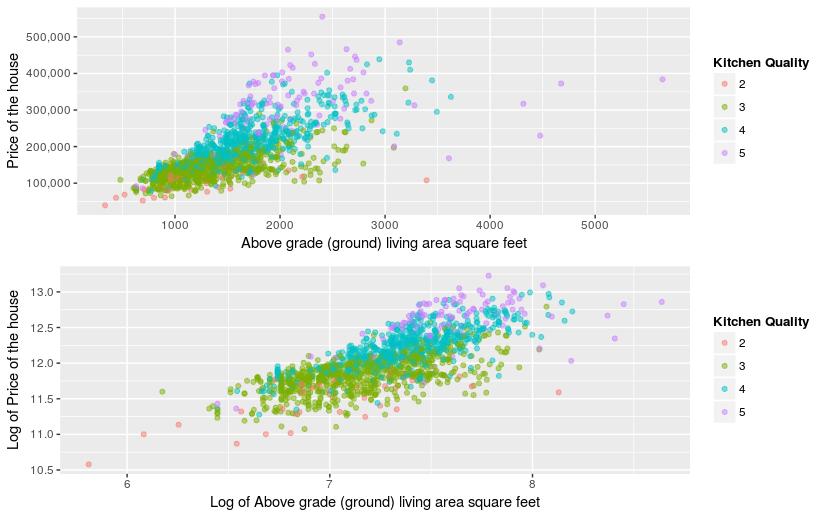
\includegraphics[scale = 0.5]{plot1.png}

\begin{flushleft}
We start out by plotting two of the best predictors of house price -- kitchen quality and above grade (ground) living area square feet. In the top graph, we see that there is a fan-shape, which indicates homoscedasticity. This is why we decided to take the log of both the explanatory and response variable to solve this problem. So, in the bottom plot, we see a fairly linear trend. As kitchen quality improves, the price of the house, on average, will also increase. Many of the houses fall within 3 or 4, which makes sense since it indicates the middle range. Furthermore, although obvious, as the square footage increases, the price of the house will also increase. 
\end{flushleft}

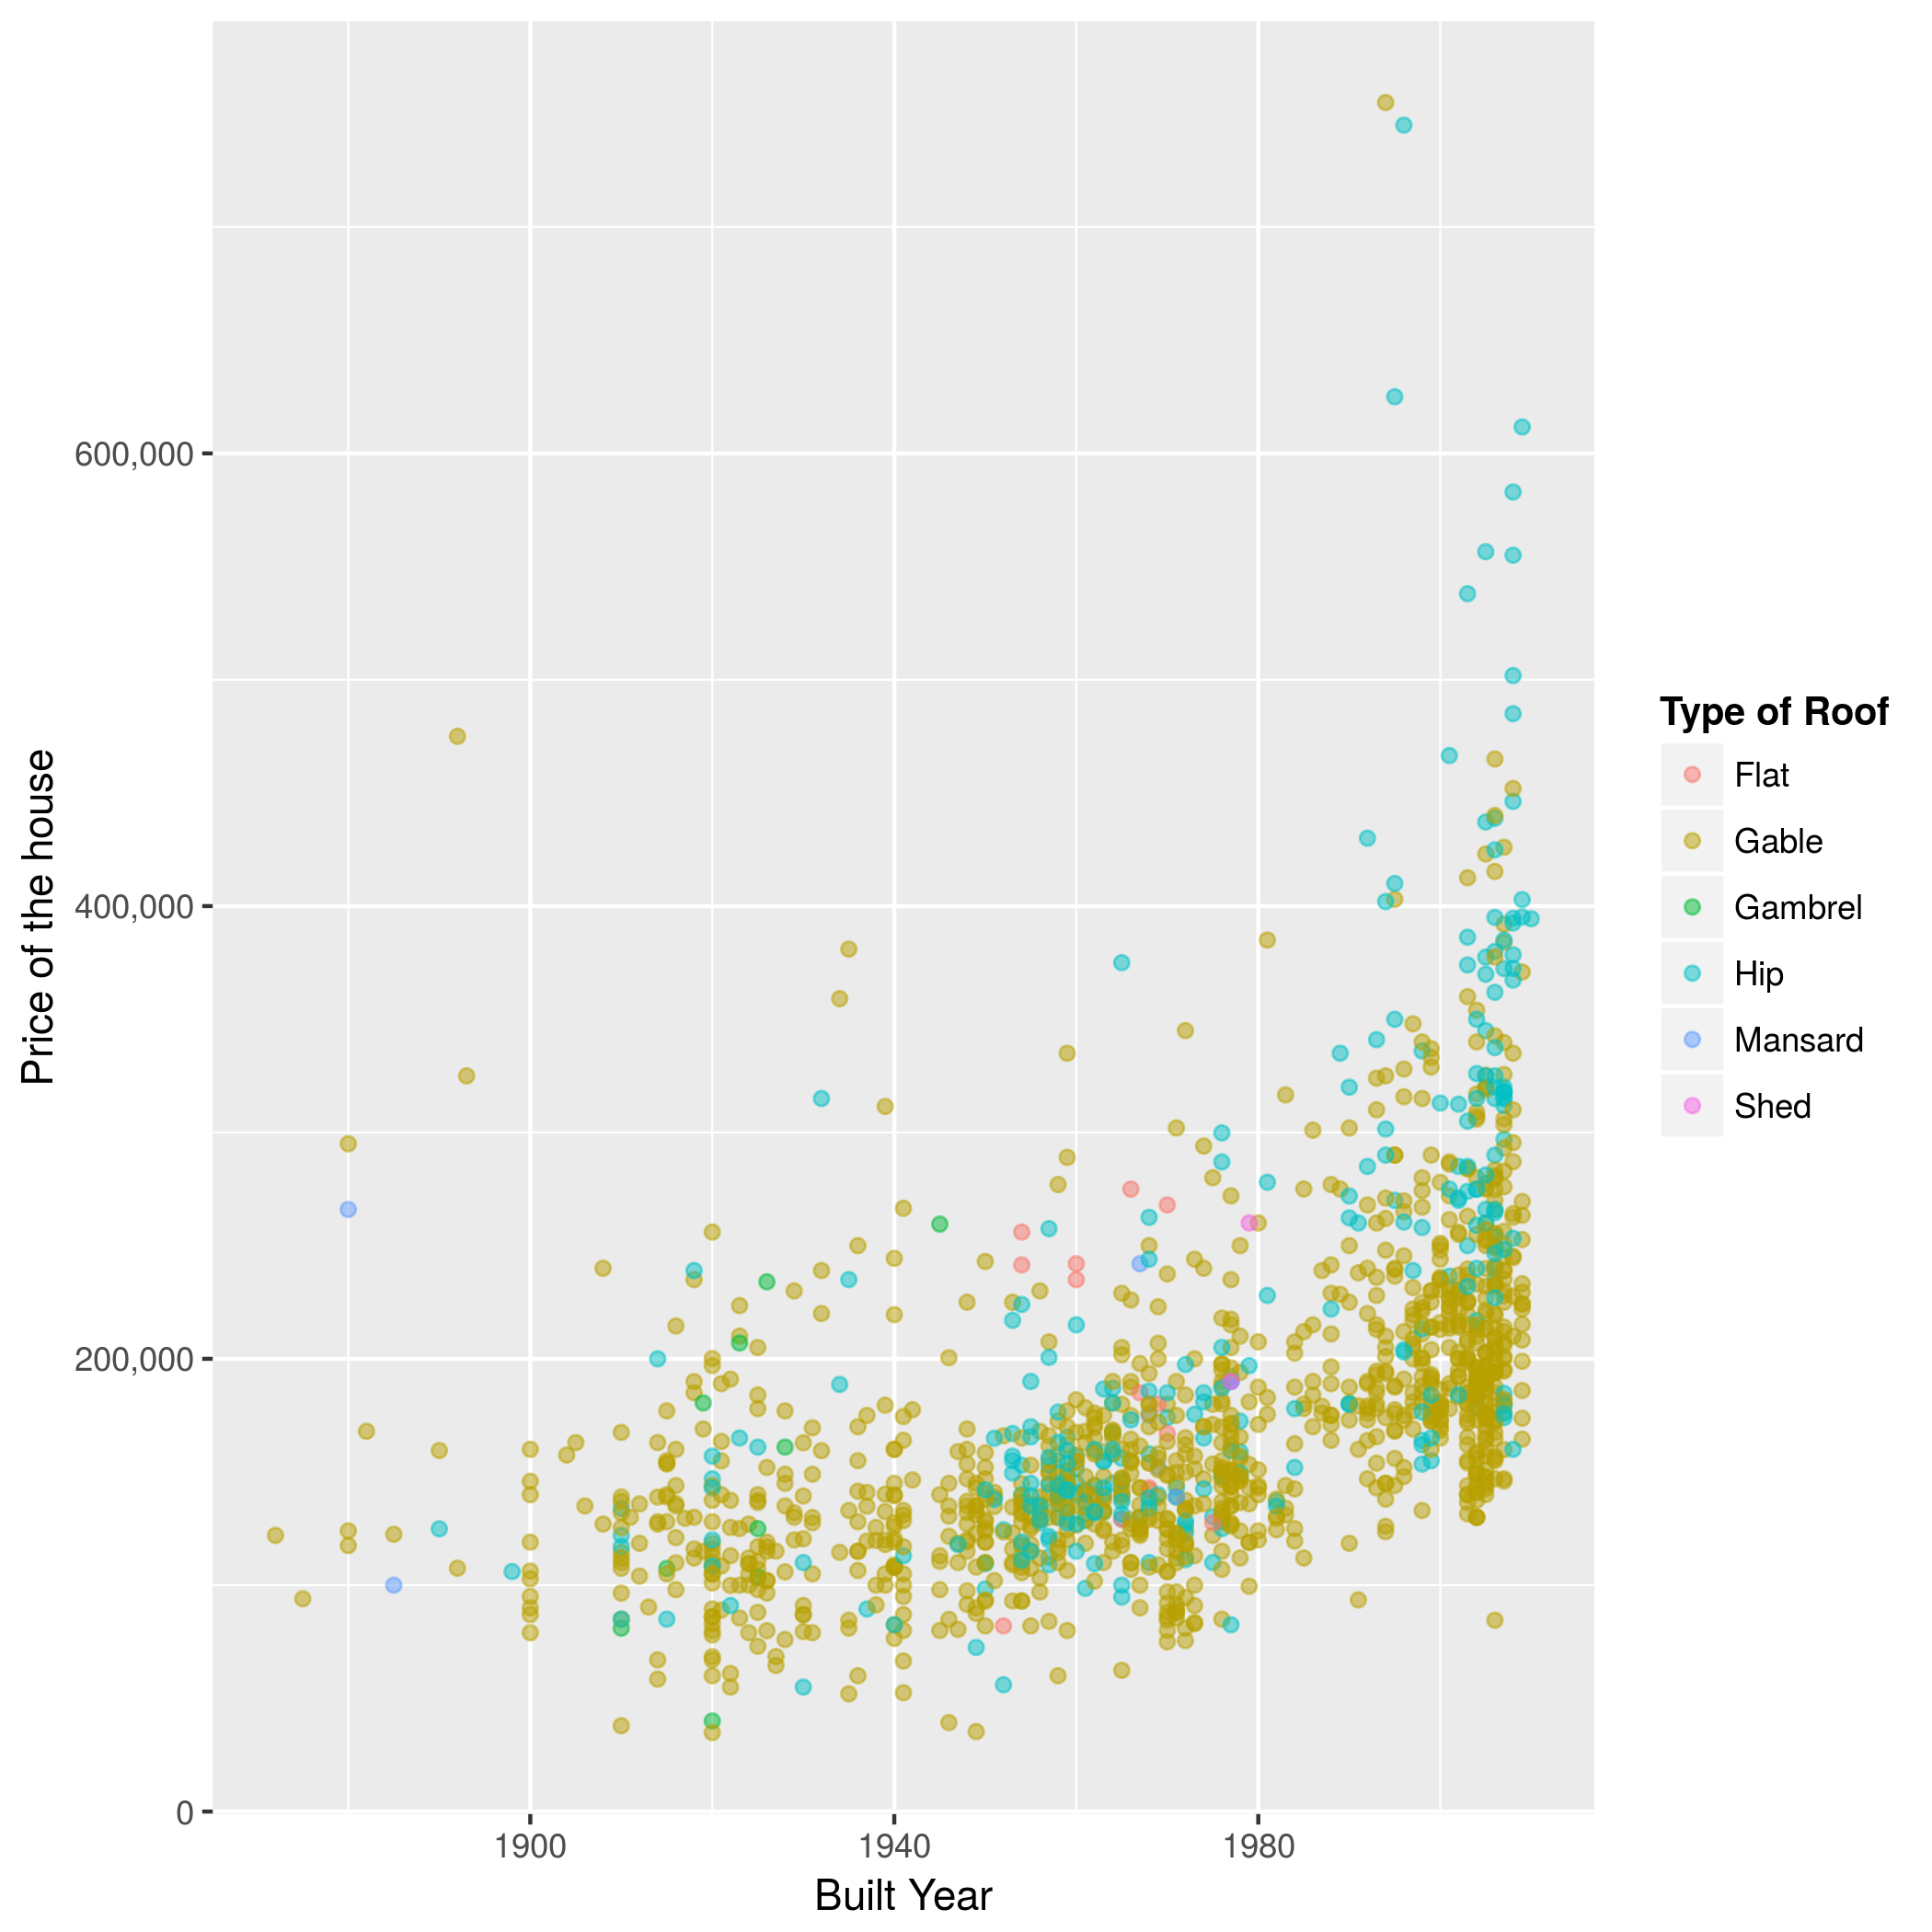
\includegraphics[scale = 0.37]{plot2.png}

\begin{flushleft}

This plot displays the price of houses over time, categorized by the type of roof. We can see that an overwhelming majority of houses are Gable houses. Hip houses are also somewhat common. In the 1960s, we see some Flat houses (in red). Throughout time, we see a general increase in the price of Hip houses over that of Gable houses. In particular, many of the extremely expensive houses are Hip ones. Most of  the houses are under \$ 200,000 but there seems to be an increase in the past years, which may just be due to inflation.
\end{flushleft}

\section{Data Processing}

\begin{flushleft}

We begin by loading the data and then taking care of any missing values. First, although the variable mssubclass appears as an integer, it is actually a categorical variable where each integer is mapped to a type of dwelling, i.e. 20 represents one-story houses after World War II. Then, we examine the number of missing values for each variable.

\begin{center}

\begin{tabular}{ |c|c|c|c|c|c|c|c|}
\hline
poolqc & 1453 & \color{red}{lotfrontage} & \color{blue}{259} & garagecond & 81 & \color{red}{bsmtfintype1} & 37\\ 
miscfeature & 1406 & garagetype & 81 & bsmtexposure & 38 & masvnrtype & 8\\
alley & 1369 & \color{red}{garageyrblt} & 81 & \color{red}{bsmtfintype2} & 38 & \color{red}{masvnrarea} & 8\\
fence & 1179 & garagefinish & 81 & bsmtqual & 37 & electrical & \color{blue}{1}\\
fireplacequ & 690 & garagequal & 81 & bsmtcond & 37 & &\\

\hline

\end{tabular}
\end{center} 

For the numeric variables (in red), we use common sense to change them to just zero. For the categorical variables, even though they were coded as missing, looking at the data dictionary, we see that NA actually means "None". In other words, for example, in poolqc, it simply means that many of the houses did \textit{not} have a pool. Because NA can be quirky in R, we change all of these missing values simply to the string "None". \newline 

Two of the variables (in blue) do not specify NA in the data dictionary. Also, by common sense, lotfrontage, which represents linear feet of street connected to property, should not be zero or missing! It is essentially saying that the house does not have a street next to it! The most likely scenario was simply that the variable was not recorded at the time. By a similar logic, every house has an electrical system and if only one value is missing, it is most likely due to an error. \newline

To solve this problem, we will apply a machine learning algorithm known as K-Nearest Neighbors. In a nutshell, this algorithm will look at the other variables for the particlar observation and make its best judgement on what the value \textit{should} be. To find the optimal k, we will use a general rule of thumb where k is the following:

$k = \sqrt{\frac{N}{2}}$ 

N represents the number of samples in our training set. We choose to split our training and testing by 80-20, making our k = 17. 

Next, we create two new variables. One , called remodel, is a boolean that indicates whether or not remodeling took place. The second, called soldminusbuilt, indicates the number of years that it took for the house to get sold after getting built. 

There are many porch variables, so we convert the porch areas all into one. Most of the houses only have one type of porch (a few observations have two types, though). 

The variable lotshape indicates whether or not the general shape of the property is regular or not. There are a few types of irregularities but because the more extreme irregularities have very few observations, we simply turn the variable into a boolean, indicating whether or not the shape is Regular or not.

\centering
    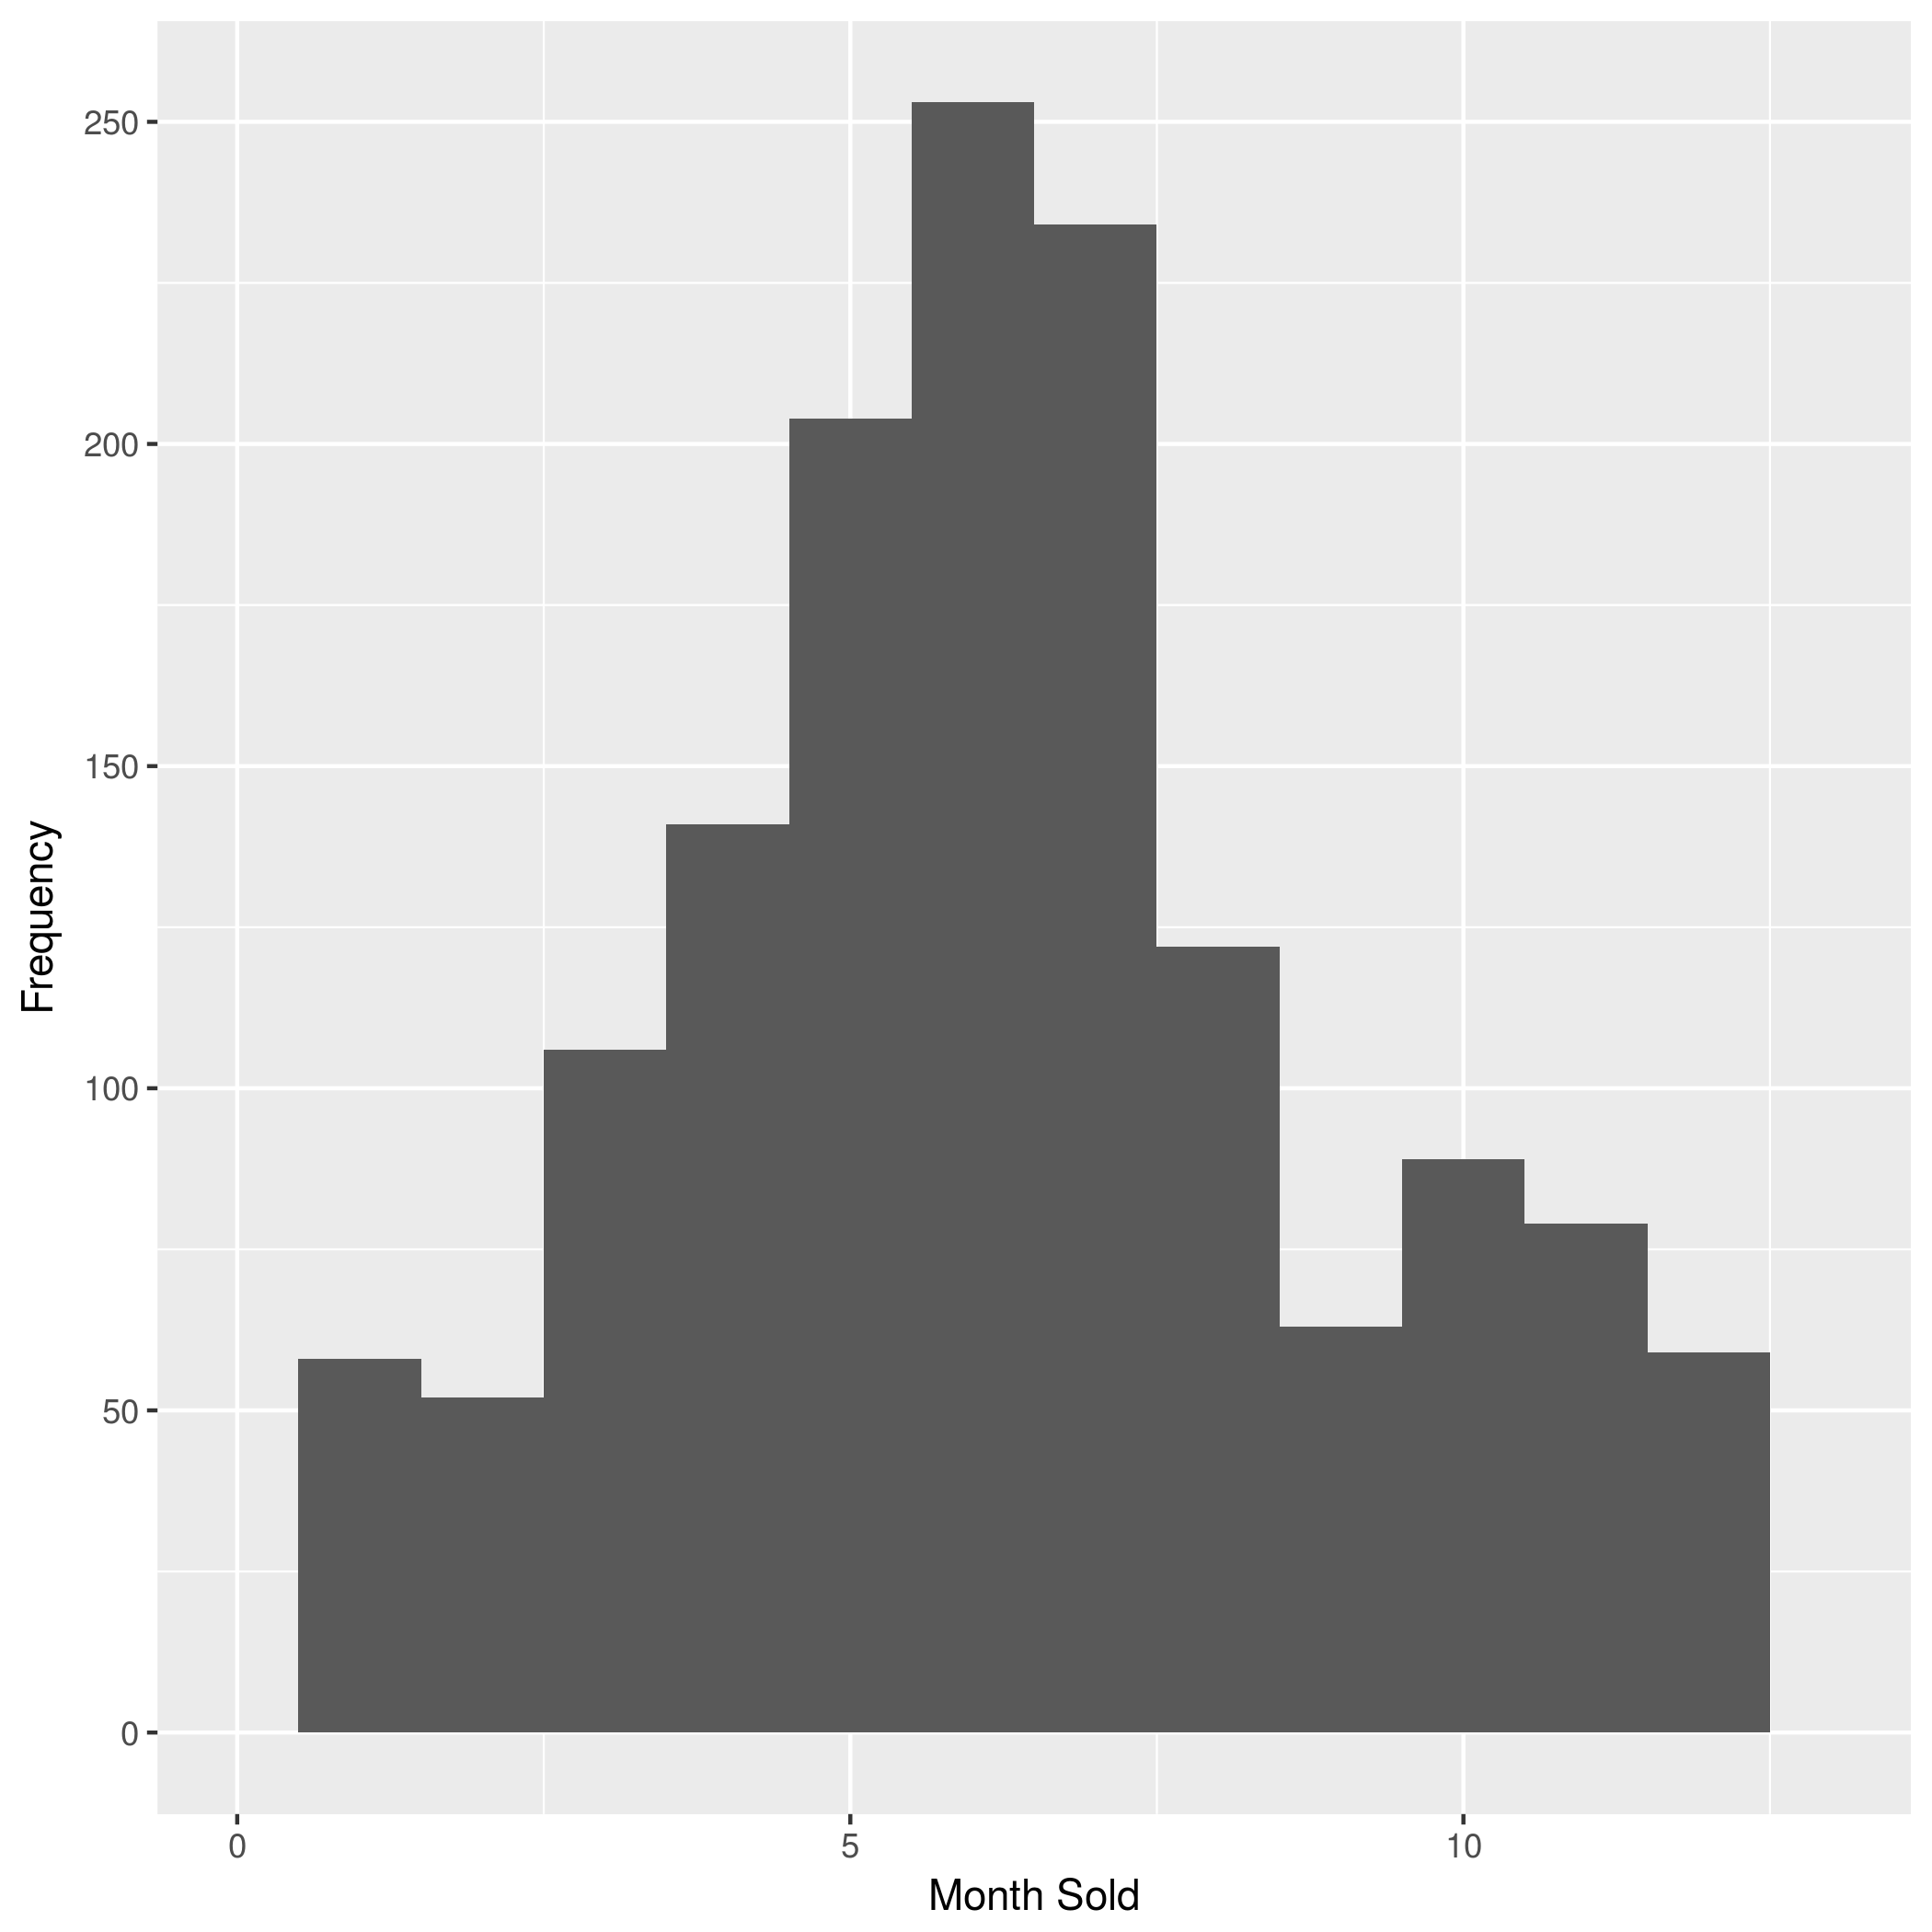
\includegraphics[scale = 0.5]{plot3.png}\\[1.0 cm]
\end{flushleft}
\begin{flushleft}
Looking at the histogram of mosold we see many more houses being sold near summer time so we create a boolean. Most of the time, when we are creating a boolean, it is because the individual levels are insignificant otherwise.



\section{Building the Model}

We perform a method that is similar to backwards selection (though manually). We start from the full model and remove insignificant variables one by one. The steps are as follows:
\begin{enumerate}

\item Check the p-value and signifiance for a particlar variable.
\item (For Categorical) Use the table function to group the counts and/or hist function to make a quick histogram. 
\item (For Categorical) Use dplyr and group\_by to look at the median price for each category.
\item If the variable is numeric and significant, keep it. If the variable is categorical and all levels are significant, keep it. If only some levels are significant then try to bin the factors into smaller number of levels to try and make them statistically significant. If nothing can be done, then remove the variable.
\item Repeat steps 1 through 4 for the rest of the variables. Each time we remove a variable, we re-run the lm model to check if the Adjusted R Squared changed significantly or not. If it decreased, we may add the variable back.
\item When we finish going through all the variables, there will be about 30 ones left to consider.
\item Stop when every single variable becomes statistically signifcant under an $\alpha$ level of 0.05. Confirm results variable selection via LASSO.
\end{enumerate}

\subsection{Notes}
\begin{itemize}
\item The variable grlivarea is equal to the sum of the variables 1stflrsf, 2ndflrsf, and lowqualfinsf. At first, we tried having all three of them and deleting grlivarea however we found that having just grlivarea performed better.
\item We modified the reference levels for the categorical variables to the most logical and/or most common level.
\item We changed ordered factors to numeric, e.g. None, Po, Fa, TA, Gd, Ex 
\item If two variables are obviously correlated with each other, we choose the variable that has a higher correlation with sales price.
\item After processing the variables, everything becomes numeric. The only categorical variable left is Neighborhood.
\end{itemize}

\section{Visualizing Correlation}

\centering
    \vspace*{0.5 cm}
    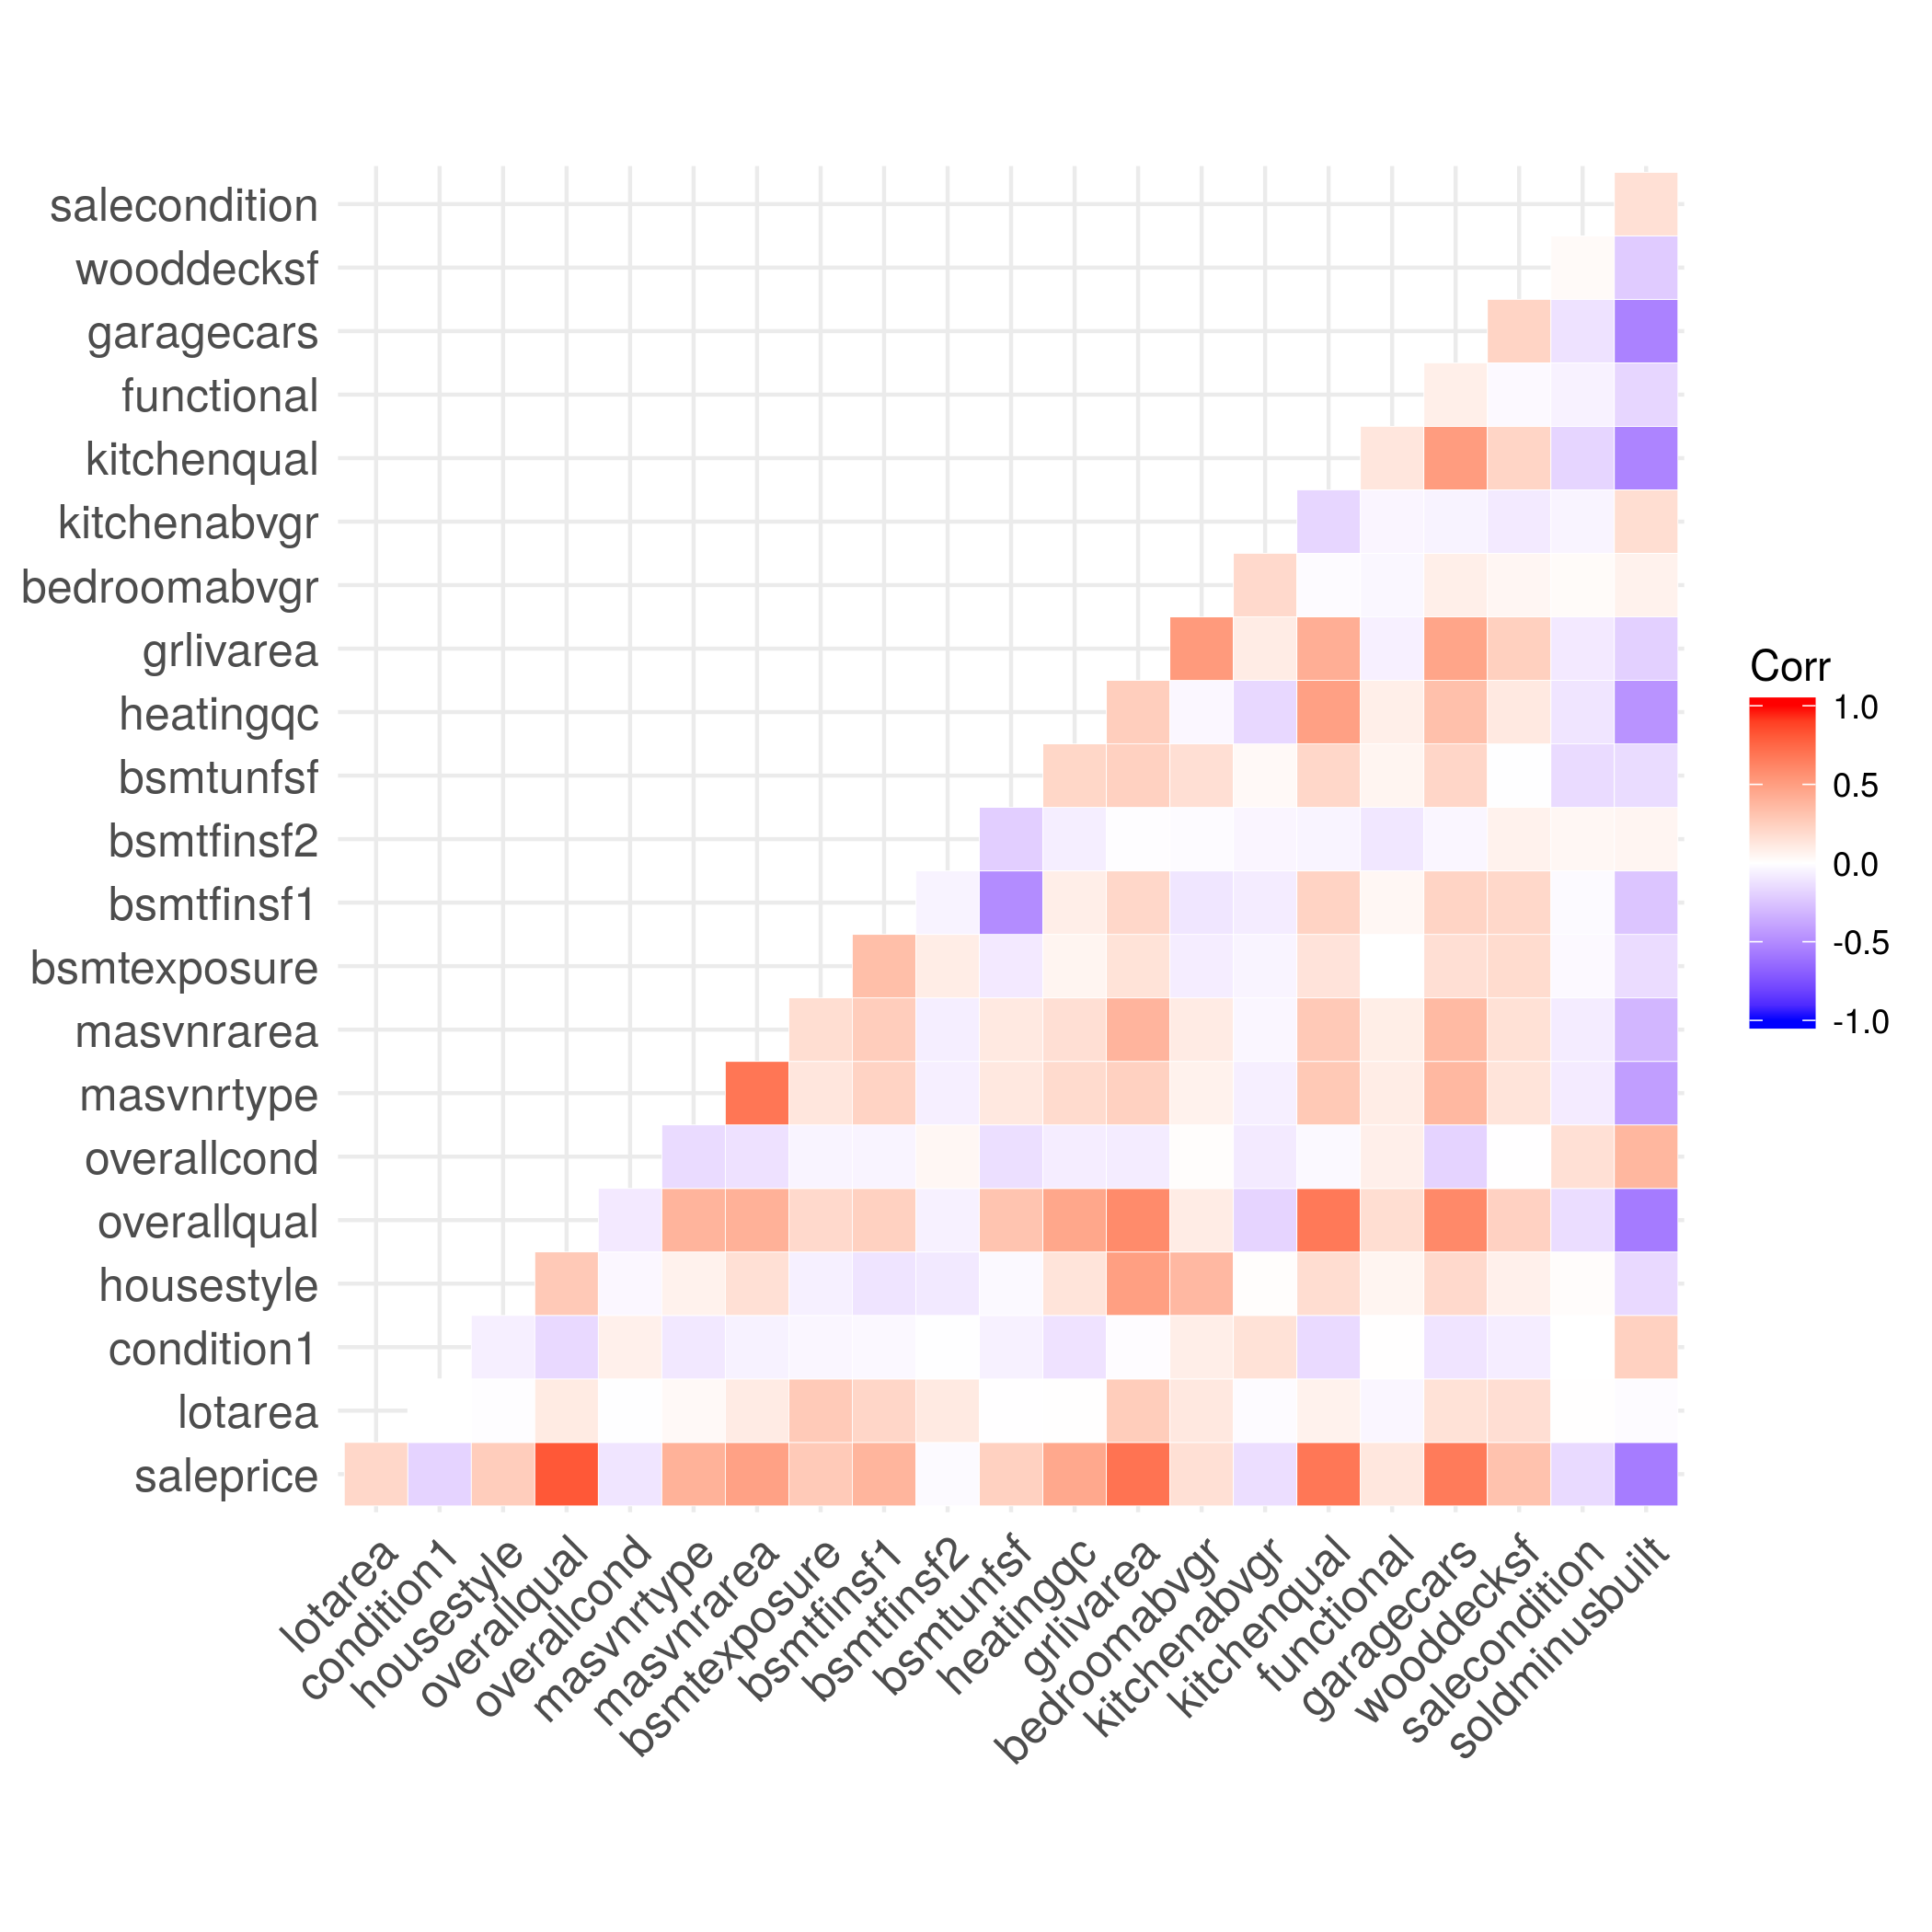
\includegraphics[scale = 1]{plot4.png}\\[1.0 cm]	% University

\end{flushleft}

\begin{flushleft}

Looking at the bottom of the correlation plot, we see how correlated each variable is to the response variable, sale price. \textbf{In particular, the most correlated variables are overallqual, grlivarea,
kitchenqual, garagecars, and soldminusbuilt. These are the most significant predictors in predicting a house price.} With only these 5 variables in the model, they explain 83.8\% of the variation in the sale price of a house!!

\end{flushleft}
\begin{flushleft}

\section{Multicollinearity}
\section{Normality}
\section{Influence Points and Outliers}

\section{Transformations}
\section{Valuation of Morty's House}
\section{Predictive Modeling}
\end{flushleft}

\end{document}